% This is samplepaper.tex, a sample chapter demonstrating the
% LLNCS macro package for Springer Computer Science proceedings;
% Version 2.20 of 2017/10/04
%
\documentclass[runningheads]{llncs}
%
\usepackage{graphicx}
\graphicspath{ {./img/} }

% copy the file from this repo
% Used for displaying a sample figure. If possible, figure files should
% be included in EPS format.
%
% If you use the hyperref package, please uncomment the following line
% to display URLs in blue roman font according to Springer's eBook style:
% \renewcommand\UrlFont{\color{blue}\rmfamily}

\begin{document}
%
\title{Ants-Review: A Protocol For Open Anonymous Peer-Reviews}
%
%\titlerunning{Abbreviated paper title}
% If the paper title is too long for the running head, you can set
% an abbreviated paper title here
%
\author{Bianca Trovò\inst{1,2}\orcidID{0000-0002-6776-2304}\thanks{Corresponding author}\and
Nazzareno Massari\inst{3,4}\orcidID{0000-0002-6638-2174}\thanks{Corresponding author}}
%
\authorrunning{B. Trovò et N. Massari}
% First names are abbreviated in the running head.
% If there are more than two authors, 'et al.' is used.
%
\institute{Sorbonne Université, Faculté des Sciences et Ingénierie, 75005 Paris, France \and
Neurospin research center, CEA/SAC/DSV/I2BM, 91191 Gif-sur-Yvette, France
\email{bianca.trovo@alumni.unitn.it}\\
\and
Alma Mater Politecnico di Torino, 10129 Turin, Italy\and
Blockchain Engineer, London, UK \\
\email{nazzareno@nazzarenomassari.com}}
%
\maketitle              % typeset the header of the contribution
%
\begin{abstract}
Peer-review is a necessary and essential quality control step for scientific publications but lacks proper  incentives. Indeed, the process, which is very costly in terms of time and intellectual investment, not only is not remunerated by the journals but it is also not openly recognized by the academic community as a relevant scientific output for a researcher. Therefore, scientific dissemination is affected in the timeliness, quality and fairness. Here, to solve this issue, we propose a blockchain-based incentive system that rewards scientists for peer-reviewing other scientists’ work and that builds up a reputational metric. We designed a protocol of smart contracts called Ants-Review that allows authors or editors to issue a bounty for open anonymous peer-reviews. If requirements are met, peer-reviews will be accepted and payed by the issuer proportionally to their quality and  constructiveness. To promote ethical behaviour and inclusiveness the system could implement a gamified mechanism that allows the whole community to evaluate the peer-reviews, vote for the best ones and share the incentives with the referees.
\keywords{Blockchain  \and Open Science \and Peer-review \and Incentivization.}
\end{abstract}
%
%
\section{Introduction}
From its birth in 2008 as a distributed ledger for the peer-to-peer electronic cash system Bitcoin \cite{BitcoinSatoshi}, blockchain technologies (BCTs) have spread far beyond the sole cryptocurrency domain, in particular after the implementation of a general purpose smart contract functionality introduced by Ethereum \cite{Ethereum}.
Besides a growing number of applications ranging from business, healthcare, music industry, government, identity to cite but a few, blockchain technology has recently started to catalyse the attention of the scientific community as well \cite{Bitcoin-Nature-focus,vanRossum2017-DigSci} with the promising potential of being a 'game changer' in outdated and broken scientific practices and leading towards Open Science \cite{AES}. Indeed, scholars have pointed out how the intrinsic characteristics of blockchain technology set the basis for a open science infrastructure \cite{ReviewBlockchain2019} where decisional processes are transparent and therefore more democratically accessible to all the stakeholders (researchers, reviewers, funders, taxpayers). Those are: \emph{consensus algorithm}, a deterministic computational trust that allows \emph{decentralization}, for which there are no trusted third parties; \emph{cryptographic hashing} and \emph{timestamping}, that create a digital footprint able to keep a traceable chronological record of research objects; \emph{immutability} or \emph{append-only}, for which data cannot be altered or retrieved. In particular, a 'blockchainified science'\cite{BlockchainforScience} could 'reduce waste'\cite{ReducingWaste-Lancet}, by disclosing each step in the research cycle to 'scientific self-correction' way before the final publication step and therefore help fixing the current reproducibility crisis in science.
\newline A thorny issue in the academic system that can and should be tackled by blockchain concerns the status and accreditation of peer-review, the core process of scientific validation currently facing a crisis \cite{Gropp-PeerRevStress}.
In this paper we propose a solution to the problem of reviewers recognition based on the principles of token economy and in line with the values of Open Science.

\section{Background}
\subsection{Peer-review: present problems and mild solutions}
Peer review is still the only quality control mechanism devoted to evaluate scientific outcomes. The purpose of peer review is "improving the quality of the published paper, determining the originality of the manuscript, determining the importance of the findings, detecting fraud, and detecting plagiarism." \cite{Gropp-PeerRevStress}. However, the system is 'flawed' and outdated \cite{Smith2006} and presents multifaceted issues, here reviewed.
\paragraph{A slow multi-stage process.} The main issues affecting the effectiveness of peer-review is the delay between paper submission and journal acceptance for publication. The traditional peer-review process is completely controlled by the editor(s). The author(s) submit manuscript to the journal where an editorial team assesses if the paper meets the scopes of the journal and novelty criteria. If the editorial decision is to send the manuscript for review, the handling editor personally selects potential reviewers. The reviewers identity is usually only known to the editor but is hidden to the authors or the other reviewers themselves (single-blind review). Reviewers independently conduct their reviews by exposing in their reports strengths and weaknesses of the manuscript and sometimes substantially improving the draft. Depending on if the decision is a major or minor revision, authors are invited to re-submit a corrected or improved version of the manuscript with a letter to the reviewers. The same reviewers might be contacted again to continue the same peer-review process. This process can take multiple rounds and is a huge time investment both for authors and reviewers. An analysis of all papers published in PubMed for a time period of 30 years claims that the median review time is around 100 days\cite{Kendall-peerrev}.
\paragraph{Lack of recognition.} Peer-reviewing is an invisible activity purely conducted on voluntary basis, neither paid by the journals or officially credited via standard scientific metrics (such as the ones that establish the 'impact factor' of an author). Thus, it does not lead to advancements in career or help securing grants. Researchers are motivated to do peer-review by a sense of belonging and a desire to 'give back' to the community. A major consequence of not promoting incentives for the quality (and quantity) of peer-reviews is to either slow down publication of potentially good research which awaits for validation or let bad science be published through sloppy and uncritical reviews.
\paragraph{Fraud and misconduct.} Due to the 'publish or perish culture' pressures, unethical behaviour from reviewers has been occasionally reported, from abusive behaviour towards authors \cite{Smith2006,tragedy-reviewers} to identity fraud. Some studies have reported an improvement in the transparency and civility of the review process when open reports are released according to the standards of open peer review.
\paragraph{Social and cognitive biases.} Given the fact that anonymity is usually asymmetrically applied only for reviewers, many power related dynamics can influence the reviewers decision, such as gender or cultural discrimination and social prestige of the institution. To solve this problem some journals have implemented double-blind review process (identity of both authors and reviewers are masked) which seems to reduce the bias towards minorities.
\paragraph{Peer reviews need to be...reviewed.} There is high variability in the reliability and depth of reviews and a recurrent question is: "Who watches the watchers?".
\paragraph{Need for more reviewers.} There is a disproportion between the progressive increase in journals publications and the number of experienced reviewers selected for the task which demands an expansion of the reviewer's pool including early career scientists. \cite{tragedy-reviewers}.

\subsection{Related work} Some mild attempts to credit peer review have been handled without much success by journals via attribution of virtual 'badges', certificates of performance, citation in annual editorials.
\newline It's also worth mentioning \emph{Publons}\footnote[1]{\emph{Publons}.\textsc{URL:} https://publons.com/about/home.}, a service integrated with ORCID (researcher identifier) that provides peer-review metric; \emph{Peerage of Science}\footnote[2]{\emph{Peerage of Science}.\textsc{URL:} https://www.peerageofscience.org.} and \emph{ResearchSquare}\footnote[3]{\emph{ResearchSquare}.\textsc{URL:}https://www.researchsquare.com.}, a journal-independent free service for scientific peer review and publishing that provides also a peer-review of the reviews. Spearpoint\cite{ResearchCoin} proposes \emph{r-coin} (for ‘ReviewCoin’ or ‘ResearchCoin’), a cryptocurrency that researchers earn for undertaking peer-reviews and that can used to pay for publication fees. \emph{ScienceMiles} \cite{ScienceMiles} is a cryptocurrency for incentivizing peer-reviews through a blockchain-based platform and an open peer-review process. Avital \cite{AvitalToken} suggests a token-based peer-review payment system. \emph{INFINITCODEX (I8X)} \cite{I8X}, is a platform that promotes cooperative user behaviour through dynamic research papers that undergo  continuous peer review process. The system implements cryptoeconomical incentives for building reputation in the community of users. \newline Other proposals to improve the peer-review system have instead focused on features such as decentralization \cite{DecentralSc2,DecentralSc1}, security \cite{Pevo,CryptSubmit,MarsChain}.

\section{System concept}
In this paper we propose Ants-Review, a new incentivisation mechanism built on a distributed platform that issues open peer-reviews to validate scientific papers while preserving the anonymity of its contributors. We imagine a final paper originating from the peer-review process as a complex system that emerges from the interactions between the authors and the reviewers, a whole that is more than the sum of its parts. Therefore, the name evokes an ant colony as a self-organising organism in which all micro-contributions of the individuals emerge into complex behaviour.
\newline The original proposal behind this paper can be found here \cite{AntsReview}.
\newline Its design and implementation are exposed in the following section.

\subsection{Design}

Here we describe the main features of Ants-Review.
\paragraph{Incentivisation and recognition.} A typical business model for open source software (OSS) movement is open-source bounty. Bounties are a prize or monetary reward given for completing a task before a deadline \cite{BountyGit}. Examples of such platforms that allow funders (bounty backers) to pay developers (bounty hunters) for open source contributions are \emph{Gitcoin}\footnote[4]{\emph{Gitcoin}.\textsc{URL:} https://gitcoin.co.} and \emph{The Bounties Network}\footnote[5]{\emph{The Bounties Network}.\textsc{URL:}https://bounties.network.}. Incentives can be cryptographic tokens, unit of values registered on a blockchain network and that represent the quantity and quality of a service within a network.
\newline In the network of the scientific community reviewers provide a service and those who consume it (authors, journals)  should be able to contribute with tokens, an internal cryptocurrency that can be spent externally. The amount of tokens reflects material and symbolic recognition of the performed work that can be statistically quantified for author-level metrics measuring the productivity and impact of a researcher.
Thus, the system acts also as a reputation builder.
\newline Moreover, to encourage commitment, reviewers who contribute consistently to multiple rounds of reviews on the same manuscript can have their tokens accrue interest over time (see 3.2).

\paragraph{Transparency and re-usability of the records.} The peer-review history, including authors' replies and editors' recommendations, should be openly and permanently accessible to the community (in the form of 'open reports' of open peer-reviews) even before articles' publication in order to  make editorial decisions more democratic and prevent waste of knowledge. Following the example of models offered by journals peer-review consortia, such as the \emph{Neuroscience Peer Review Consortium}\footnote[6]{\emph{Neuroscience Peer Review Consortium}.\textsc{URL:}http://nprc.incf.org.} and independent companies like \emph{ResearchSquare}  and \emph{Peerage of Science}, peer-reviews in Ants-Review will be transferable across journals (like in 'cascading' or 'portable peer-reviews').

\paragraph{Accountability via pseudo-anonymity.} In order to counteract malicious behaviour (see 2.1) affecting the integrity of the reviews but also to correctly attribute the intellectual contributions making sure there are no conflict of interest, it's important to be able to track back the identities of the contributors to a peer-review report. This is possible if the platform acts like a version control system where commits are permanent and their hashes timestamped. InterPlanetary File System (IPFS) \cite{IPFS} is a peer-to-peer hypermedia protocol for storing data in a distributed file system over the internet which guarantees data \emph{immutability} and unique file identification via cryptographic hashes. IPFS' hashes are then stored inside the smart contracts' state that is timestamped into the Ethereum blocks where  the transactions take place; there, data remain unaltered and indelible. This notarization process is called Proof of Existence (PoE)and allows manual verification of the existence of the document.
\newline To prevent retaliation for negative peer-reviews and to promote the participation of early researchers who might feel intimidated to judge the scientific work of senior authors, the Ants-Review system maintains the privacy of both authors and reviewers in a double-blind approach via Ethereum’s Externally Owned Accounts(EOA) addresses, zero-knowledge proofs, a cryptographic method where a party can prove to another party the possession of certain information, like a secret key, without revealing that information (see § Privacy in 3.2).

\paragraph{Inclusiveness via gamification.} As a final step we propose that all the community is involved in the process of peer-reviewing abolishing the editorial selection process ('open participation', 'open interaction', 'open platform' \cite{OPR-Ross-Hellauer}). In this way, the pool of reviewers is enriched and allows younger researchers to get the appropriate training through interactive feedback. Moreover, peer-reviews could be evaluated, commented, criticised by the other members of the scientific community, enabling a virtuous loop of verification. \newline An interesting addition would be to introduce Quadratic Voting (QV) \cite{QVWeyl} for the reviews' evaluation. QV replaces the discrete concept of one-person-one-vote with the non-linear one of n vote at the cost of $n^2$ and is optimal in the context of multiple choices. If we consider scientific outputs as public goods, then the community can vote (with voting tokens) 'how much they care' for a specific peer-review. A rank of peer-reviews would result from the voting process, with a more fine-graded distribution that might reflect issues that have a high value to few people and low value to more people. \newline Finally, it's conceivable that the members of the community participate to the share of the tokens by voting to the best peer-reviews. This solution would create a self-reinforcing ethical behaviour where the fair evaluation of peer-reviews would be also in the interest of the agents at play.

\subsection{Implementation}

\begin{figure}
\centering
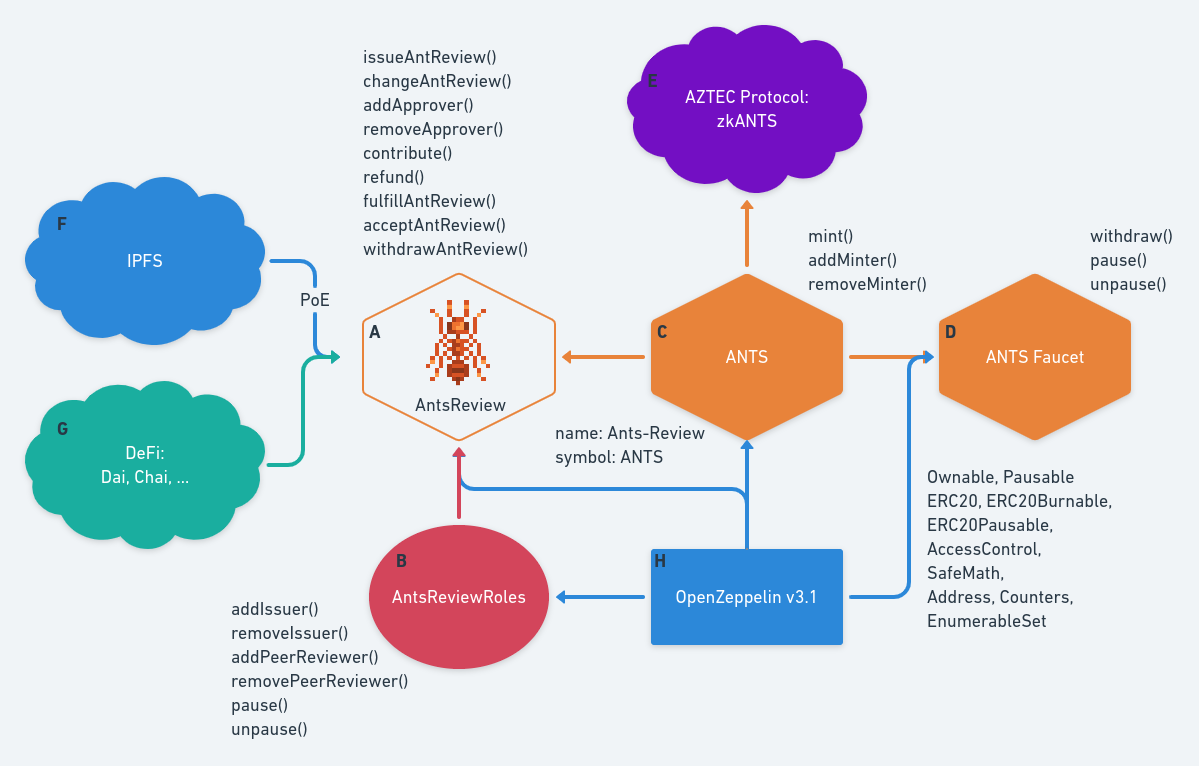
\includegraphics[scale=0.28]{Ants-Review}
\small{
\caption{Exagones represent the protocol's smart contracts. Ellipse represents the smart contract inherited by AntsReview. Clouds represent integrations into the protocol. Rectangles represent smart contracts' libraries.
\textbf{a} Core contract of the protocol implementing a bounty system with the functions listed.
\textbf{b} Module inherited by AntsReview: it manages the access control of the protocol by adding and removing issuers and peer-reviewers.
\textbf{c} Native token used in the protocol. It is linked to (\textbf{a}), (\textbf{e}) and to (\textbf{d}).
\textbf{d} Faucet to distribute \emph{ANTS} on Kovan Testnet for testing purposes. 
\textbf{e} Integration with Aztec Protocol to wrap (\textbf{c}) into \emph{zkANTS} to implement private \emph{ANTS} transactions on Ethereum.
\textbf{f} Integration with IPFS to upload papers, requirements and peer-reviews and store the hash as \emph{PoE} into AntsReview.
\textbf{g} Integration with De-Fi services like \emph{Dai} and \emph{Chai}, to be used as tokens in the protocol.
\textbf{h} Library used by the protocol for secure contract development with the modules listed.}}
\label{fig:contracts}
\end{figure}

In the following sections we describe the architecture of the system and its building blocks.
\newline The Ants-Review Protocol is divided into different modules responsible for the following functionalities, as shown in the flow-chart (see Figure \ref{fig:contracts}):
\emph{AntsReview}, which manages access management and the core system (see Figure \ref{fig:contracts}, (\textbf{a, b, f, h})).
\emph{Privacy}, which maintains the anonymity of the system via AZTEC Protocol (see Figure  \ref{fig:contracts}, (\textbf{d})).
\emph{Tokenomics}, which manages the incentive mechanism of the system (see Figure \ref{fig:contracts}, (\textbf{c, e, h})}).

\subsubsection{AntsReview.}
AntsReview (see Figure \ref{fig:contracts} (\textbf{a}) is the core of the smart contracts written in \emph{Solidity}\footnote[7]{\emph{Solidity}.\textsc{URL:}https://solidity.readthedocs.io.}, a contract-oriented programming language for writing smart contracts that runs on the Ethereum Virtual Machine, deployed on Ethereum Kovan Testnet\footnote[8]{\emph{Kovan Testnet}.\textsc{URL:}https://kovan.etherscan.io/.}. AntsReview implements a bounty-like system (based on the \emph{StandardBounties} contract\footnote[9]{\emph{StandardBounties.sol}.\textsc{URL:}https://github.com/Bounties-Network/StandardBounties/blob/master/contracts/StandardBounties.sol.}) where Alice (issuer) can issue an AntReview with the function \emph{issueAntReview()}.
\newline In order to create a transparent and openly accessible AntReview, Alice has to complete a series of required tasks:
 \begin{itemize}
     \item \emph{upload of the files} containing the requirements of the peer-review and the paper to be reviewed into IPFS, whose hash is stored into the Ethereum blockchain as PoE;
     \item \emph{specification of a deadline} in the form of a UNIX timestamp after which the fulfillment will no longer be accepted;
     \item \emph{specification of the Issuers and an Approver} to respectively modify the AntReview and approve the peer-reviews sent by the peer-reviewers;
\end{itemize}
 Alice or the Issuers can at any time update the AntReview details (issuers, paper, requirements, deadline) with the function \emph{changeAntReview()} and add/remove the Approver with the functions \emph{addApprover()} and \emph{removeApprover()}.
 Anters (members of the Ants-Review Community), can contribute to Alice's AntReview with the function \emph{contribute()}, by specifying the amount of ANTS they are willing to send.
 Bob (peer-reviewer) can download the files relative to Alice's paper and requirements by leveraging on the content-addressing feature of IPFS, that allows anyone to find the document using an IPFS explorer; subsequently, Bob can submit a peer-review before the deadline by fulfilling the AntReview created by Alice, with the function \emph{fulfillAntReview()}, by uploading the peer-review on IPFS, whose hash is stored into Ethereum blockchain as PoE. He can update the peer-review with the function \emph{updateReview()} by uploading the new version on IPFS.
The Approver can accept the peer-review submitted by Bob with the function \emph{acceptAntReview()}, by specifying the amount of ANTS that will be transferred as reward from the contract to Bob.
If Alice's AntReview does not receive any peer-review and the deadline expires, Anters can get a refund with the function \emph{refund()} for their contributions. In order to avoid residual balance, Alice can withdraw ANTS from the AntReview's balance, if the deadline expires, with the function \emph{withdrawAntReview()}, and the contract will transfer the amount specified to Alice and update the balance.

Access management of the Ants-Review protocol is defined and controlled by AntsReviewRoles (see Figure \ref{fig:contracts} (\textbf{b})), implemented by leveraging on \emph{AccessControl.sol} by OpenZeppelin Solidity Library\footnote[10]{\emph{OpenZeppelin Library}.\textsc{URL:}https://openzeppelin.com.} that it's used to define the Issuer and Peer-Reviewer Roles.
\newline AntsReviewRoles also integrates a circuit breaker design pattern via \emph{Pausable.sol} by OpenZeppelin to allow the Pauser Role, that by default is granted to the Owner of the smart contracts, to pause (or unpause) all the functions in case of a security emergency, such as an attack to the smart contracts.

\subsubsection{Privacy}
The anonymity of an agent in the system is achieved in two ways: via pseudo-anonymity, granted through Ethereum's EOAs that can pseudo-obscure the identity of the agent; via private transactions allowed by AZTEC Protocol\cite{AZTEC}'s security layer.

\paragraph{Pseudo-anonymity.}EOAs in Ethereum are controlled via private keys. However, the privacy is limited by the fact that both the blockchain and its transactions are public.  Therefore, the details of the transactions are visible to anyone by browsing a block explorer (such as Etherscan) and are subject to data mining that could extract value and identify users in the blockchain.
\paragraph{Private transactions.}AZTEC Protocol  was conceived to enable privacy on public blockchains. It uses Zero-Knowledge Succinct Non-Interactive Argument of Knowledge (ZK-SNARKs)\cite{ZKSNARKs} and homomorphic encryption\footnote[11]{\emph{Homomorphic Encryption}.\textsc{URL:}https://vitalik.ca/general/2020/07/20/homomorphic.html.} to validate encrypted transactions.
\newline ZK-SNARKs are zero-knowledge proofs that require no interaction between prover and verifier.ZK-SNARKs are used inside the Ants-Review protocol via the zkANTS token to allow private transactions between the agents (Alice & Bob).
\newline Future developments will allow to leverage on Permutations over Lagrange-bases for Oecumenical Noninteractive arguments of Knowledge (PLONK) \cite{PLONK}proofs, a universal ZK-SNARK construction that reduces gas costs and improves scalability.

\subsubsection{Tokenomics}
Ants-Review integrates a few \emph{ERC20}\footnote[12]{\emph{EIP 20}.\textsc{URL:}\url{https://eips.ethereum.org/EIPS/eip-20}.} tokens, each of which plays an integral role in the functioning and anonymity of the decentralized protocol.
\newline ANTS (see Figure \ref{fig:contracts}, (\textbf{c})) is the primary protocol token and can be staked into an AntReview.
\newline ANTS is implemented by inheriting \emph{ERC20PresetMinterPauser.sol} from OpenZeppelin Library with name \emph{Ants-Review} and symbol \emph{ANTS}.
\newline zkANTS (see Figure \ref{fig:contracts}, (\textbf{d})) is a wrapper of ANTS that will be used inside the protocol to allow private transactions among the agents, preserving their anonymity as well as the amount of the AntReview reward and the contributions by the Anters. zkANTS will be implemented via AZTEC Protocol \cite{AZTEC}, that uses a cryptographic engine, \emph{ACE.sol}, a contract responsible for validating the set of AZTEC zero-knowledge proofs and performing any transfer instructions involving AZTEC notes, minted into a zkAsset, that can be converted into ERC20 tokens. In order to implement a zkAsset called zkANTS, \emph{zkAsset.sol}, a contract implementation of a confidential token that follows the EIP-1724 standard \footnote[13]{\emph{EIP  1724}.\textsc{URL:}\url{https://github.com/ethereum/EIPs/issues/1724.}}, will be used as template to build an AZTEC-compatible asset.
\newline To optimize and scale transactions, AZTEC Protocol ZK-SNARKs, will be extended in the future to PLONK \cite{PLONK} to collapse the gas costs of private transactions.

\section{Discussions}
We have described how Ants-Review protocol can solve the limitations of the current peer-review system (see 2.1). In particular we showed how the lack of recognition, the lack of transparency, fraud and misconduct can be solved via the Ants-Review Protocol (see § AntsReview in 3.2); social and cognitive biases via anonymity granted by AZTEC Protocol (see § Privacy in 3.2); the slowness of the process, the need for evaluation of the peer-reviews themselves and the need for increasing the number of reviewers by the creation of the community of Anters.
\subsection{Future developments}
The Ants-Review Protocol will make the following integrations.
An interesting aspect of the protocol is the double function of an AntReview that is a the same time a bounty and a pool to stake ERC20 tokens. Therefore, the duration of peer-reviews consents to connect the protocol to De-Fi services, such as Dai\footnote[14]{\emph{Dai}.\textsc{URL:}https://docs.makerdao.com/smart-contract-modules/dai-module/dai-detailed-documentation.}, Chai\footnote[15]{\emph{Chai}.\textsc{URL:}https://chai.money.}, with the possibility of accruing interest over time via MakerDAO DSR (Dai Saving Rate)\footnote[16]{\emph{Pot}.\textsc{URL:}https://docs.makerdao.com/smart-contract-modules/rates-module/pot-detailed-documentation.} or Compound\footnote[17]{\emph{Compound}.\textsc{URL:}https://compound.finance.} to cite a few. 
In particular, we are considering to implement another ERC20 token, called \emph{Hive}, symbol \emph{HIVE}, a wrapper of ANTS that represents the accrued interest of the Anters' stake into AntReviews.
This token doesn't need to be locked in the network and it can be traded, sold, or held as the Anter desires.
A Decentralized Autonomous Organization (DAO) could be formed in the future to allow ANTS stakers to participate in the governance of important aspects of the protocol, from smart contracts upgrades to minor changes in settings across the protocol.
\newline Finally, another concept under investigation is Quadratic Funding \cite{LiberalRadicalism}, used by \emph{Gitcoin} to match donations for grants. This will allow to incentives prolific peer-peviewers and research and improve the stability of the system together with ideally a reward system to rank the best peer-reviewers.

\subsection{A new community-driven standard?}
As Tennant points out\cite{Tennant2017-F1000R}, a change is already happening in the publishing industry, especially with new born publishers opening up the review process (\emph{BioMed Central}, \emph{ELife}, \emph{Frontiers}, \emph{PeerJ}, \emph{F1000 Research}). If also pre-print platforms integrate peer-review into their platforms, the dissociation of initial scientific dissemination and scientific validation will force the publishing industry to adapt in order to keep up with the higher quality scientific process offered by alternative peer-review platforms and justify their added value.
In our proposal we posed two possible integrations for Ants-Review, a simpler one which maintains part of the journals' power in the peer-review evaluation and more complex one that completely decouples the peer-review process from the publishers giving it back to the scientific community and applying concepts from mechanism design. This second option, which requires further implementations, is the one we aim at. Indeed, we foresee that the future will evolve towards community-organized peer reviews: peer reviews will be more and more independent from publishers, and researchers will be the ones seeking the papers to review to build reputation within the community and not journals.
Peer reviews requires a standard: building smart-contracts for peer-reviews might set a first step in this direction and our work seems promising. We hope that soon the value of peer review as 'academic capital' will be recognized by research funders and hiring committees.

\section{Conclusion}
In this paper we addressed a crucial problem within scholarly academic communication: the peer-review process. We've shown how blockchain technology could provide an efficient and viable solution to open up possible directions for a paradigm shift in scientific communication. We proposed an incentive mechanism that could solve the problems of lack of acknowledgment and trust during peer-reviews. We exposed the architecture of our project for which we adopted cutting-edge tools from the open source blockchain ecosystem.

\small{
\subsubsection{Supplementary material}
Source code, DOI: 10.5281/zenodo.3971044; 
\newline DApp, https://ants-review.on.fleek.co;

\subsubsection{Declaration of Competing Interest}
The authors declare no competing interests.

\subsubsection{Acknowledgements} We would like to thank Matteo A. Tambussi, Andy Tudhope, Mark Beylin, Evan C. Harris, Mitrasish Mukherjee and the external anonymous peer-reviewers.}


% ---- Bibliography ----
%
% BibTeX users should specify bibliography style 'splncs04'.
% References will then be sorted and formatted in the correct style.
%
\bibliographystyle{splncs04}
\bibliography{ref1-intro.bib,ref2-peerreview.bib,ref2-related.bib, ref3-system.bib,ref4-discuss.bib, ref5-extra.bib}

\end{document}
